\chapter{Final Result and Conclusion} \label{result}

In this chapter we show the result obtained for the \transv measured on carbon during the experiment.
The first result that we report is the values of asymmetry $\overline{A}_{n}$ computed as the average over all the events, after applying the various cut discussed before to remove wrong data and outliers. The values reported in tables \ref{table:NotCorrected} \ref{table:OffsetCorrected} are corrected by te beam polarization ($A_{raw} \times \frac{1}{P}$) and by the current asymmetry:

\begin{equation}
\overline{A}_{n} = \frac{\overline{A}_{raw}}{P} - \overline{A}_{I}
\end{equation}

The sign of the asymmetry is given by the sign of the cross product between $\vec{k}$ incident electron and $\vec{k'}$ scattered electron. The results have positive sign for detector A and negative sign for detector B, in agreement with the kinematics.
In section \ref{Autocalib} we have discussed possible effects that arise from the presence of a PMT offset when we check the linearity of the PMTs respect to the beam current variation. This systematic effect tends to decrease the reconstructed values of the asymmetry by a factor $c$, computed in equation \ref{eq:Systematic}. The predicted value of $c$ reported in table \ref{table:PMToffset}; we also compute the ratio between the final asymmetries with and without subtracting the offset, that is reported in table \ref{table:Cfactor}. The values of $c$ computed in these two ways are coherent.

\begin{table}[hbtp]
\centering
\subfloat[][\emph{Asimmetries, with offset not subtracted.} \label{table:NotCorrected}]{ 
\bgroup
\def\arraystretch{1.1}
\begin{tabular}{c|c|c}
\hline
 PMT &   $\overline{A}_{n}$ [$ppm$] &   $\sigma$ \\
\hline
 B0  &    -19.92 &      7.7 \\
 B1  &    -19.0  &      7.8 \\
 B2  &    -23.42 &      8.7 \\
 A0  &     18.8  &      3.7 \\
 A1  &     16.05 &      3.4 \\
 A2  &     18.45 &      3.7 \\
 A3  &     19.0  &      4.2 \\
 A4  &     20.84 &      5.0 \\
 A5  &     22.83 &      4.9 \\
 A6  &     17.49 &      5.5 \\
 A7  &     19.24 &      6.6 \\
\hline
\end{tabular}
\egroup
} \qquad
\subfloat[][\emph{Asymmetries with offsets subtracted}\label{table:OffsetCorrected}]{
\bgroup
\def\arraystretch{1.1}
\begin{tabular}{c|c|c} 
\hline
 PMT &  $\overline{A}_{n}$ [$ppm$] &   \sigma \\
\hline
 B0  &    -20.61 &      8   \\
 B1  &    -19.69 &      8   \\
 B2  &    -24.13 &      9   \\
 A0  &     24.55 &      4.2 \\
 A1  &     22.54 &      4.1 \\
 A2  &     24.37 &      4.3 \\
 A3  &     23.49 &      4.7 \\
 A4  &     24.21 &      5.4 \\
 A5  &     26.39 &      5.3 \\
 A6  &     19.82 &      5.9 \\
 A7  &     20.97 &      6.9 \\
\hline
\end{tabular}
\egroup}
\qquad
\subfloat[][\emph{$c$ factor, as defined in \ref{eq:Systematic}} \label{table:Cfactor}]{
\bgroup
\def\arraystretch{1.1}
\begin{tabular}{c|c} 
\hline
 PMT index   &  $\overline{A}_{not corrected}$/$\overline{A}_{corrected}$  \\
\hline
 B0    & 0.97 \\
 B1    & 0.96 \\
 B2    & 0.97 \\
 A0    & 0.77 \\
 A1    & 0.71 \\
 A2    & 0.76 \\
 A3    & 0.81 \\
 A4    & 0.86 \\
 A5    & 0.87 \\
 A6    & 0.88 \\
 A7    & 0.92 \\
\hline
\end{tabular}
\egroup}
\caption{Averaged asymmetries over all the events. The values are corrected subtracting $\overline{A}_{I}$ and considering the effective polarization $p$ of the beam}
\end{table}

The results reported in table \ref{table:OffsetCorrected} are show in plot \ref{fig:FirstVal}.
To Obtain a final asymmetry for detector A and B, the asymmetries for each plot are averaged using the formula:

\begin{equation} \label{eq:FinalValue}
A_{n} = \sum_{i = 0}^{n_{PMT}} \dfrac{ w_{i} A_{i}}{\sum_{i = 0}^{n_{PMT}} w_{i}}
\end{equation}

With $w_{i} = \frac{1}{\sigma^{2}_{i}}$. The above equation is the error-weighted mean, used to combine measurements with different statistical error. 

\begin{figure}[hbtp]
\centering
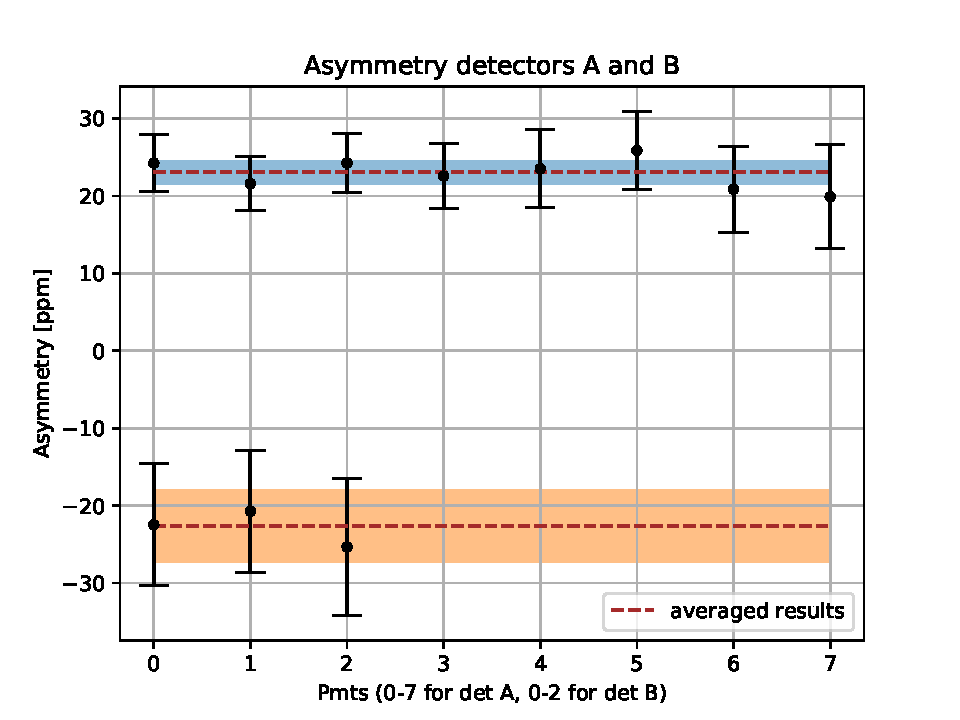
\includegraphics[width = 0.80\textwidth]{Analysis/Dataselection/FirstResult.pdf}
\caption{Plot of $\overline{A}_{n}$. The result are corrected by the beam asymmetry current and polarization. The black line represent the overall value $A_{n}$ computed with the formula \ref{eq:FinalValue}.
$\overline{\delta I}$.}
\label{fig:FirstVal}
\end{figure}

The result obtained for both the two detector are reported here. The two values are in agreement with the expected sign and compatible with the previous measurement performed at MAMI \cite{Esser:2018vdp}. 

\begin{itemize}
\item Asymmetry for detector A, $A_{A} =  23.6 \pm 1.7$ ppm.
\item Asymmetry for detector B, $A_{B} = -21 \pm 5$ ppm.
\end{itemize}

\newpage
\section{Linear Model Result}
The result obtained from the linear fit of the asymmetries versus the beam parameters are reported here, together with the false asymmetry values. The final parameters for the model are $X$, $Y$, $E$, and the current asymmetry $I$ is subtracted for each event:

\begin{equation}
A_{tot} - A_{I} = A_{n} \frac{1}{P} + A_{x} \delta X + A_{y} \delta Y + A_{e} \delta E
\end{equation}

The result for detector A: 

\begin{table}[hbtp] 
\centering
\begin{tabular}{c|c|c|c|c|c}
\hline
 PMT   & $A_{n}$    & $A_{x}$          & $A_{y}$            & $A_{e}$         & $\chi^{2}_{reduced}$ \\
\hline
 A0    & 24 $\pm$ 4 & 67 $\pm$ 27  & -8 $\pm$ 135   & -22 $\pm$ 12 & 1.000 $\pm$ 0.002   \\
 A1    & 23 $\pm$ 4 & 9 $\pm$ 26   & -85 $\pm$ 130  & -10 $\pm$ 11 & 1.001 $\pm$ 0.002 \\
 A2    & 23 $\pm$ 4 & -12 $\pm$ 27 & -24 $\pm$ 134  & -21 $\pm$ 12 & 1.000 $\pm$ 0.002   \\
 A3    & 23 $\pm$ 5 & 14 $\pm$ 29  & -180 $\pm$ 142 & -31 $\pm$ 12 & 0.999 $\pm$ 0.002 \\
 A4    & 25 $\pm$ 5 & 50 $\pm$ 31  & -85 $\pm$ 151  & -26 $\pm$ 13 & 1.000 $\pm$ 0.002   \\
 A5    & 27 $\pm$ 5 & 31 $\pm$ 31  & 198 $\pm$ 152  & -37 $\pm$ 13 & 1.001 $\pm$ 0.002 \\
 A6    & 20 $\pm$ 5 & 7 $\pm$ 33   & 142 $\pm$ 164  & -31 $\pm$ 14 & 1.000 $\pm$ 0.002   \\
 A7    & 20 $\pm$ 6 & 6 $\pm$ 38   & 78 $\pm$ 184   & -14 $\pm$ 16 & 1.001 $\pm$ 0.002 \\
\hline
\end{tabular}
\caption{Fit result with the linear model, for detector A.}
\label{tb:resultA}
\end{table}

the result for detector B: 

\begin{table}[hbtp]
\centering
\begin{tabular}{c|c|c|c|c|c}
\hline
 PMT   & $A_{n}$         & Bx         & By           & Be        & $\chi^{2}_{reduced}$\\
\hline
 B0    & -20 $\pm$ 8 & -59 $\pm$ 40 & -25 $\pm$ 187  & -14 $\pm$ 17  & 1.000 $\pm$ 0.002 \\
 B1    & -20 $\pm$ 8  & -64 $\pm$ 40 & 47 $\pm$ 188    & -22 $\pm$ 18 & 1.000 $\pm$ 0.002 \\
 B2    & -24 $\pm$ 9 & -65 $\pm$ 46 & -170 $\pm$ 211 & -61 $\pm$ 20 & 1.000 $\pm$ 0.002 \\
\hline
\end{tabular}
\caption{Fit result with the linear model, for detector B.}
\end{table}

The final results of the \transv for the two detectors, for a $Q^{2} = \SI{0.04}{\giga \electronvolt \squared}$, computed with the weighted mean are then:

\begin{table}[h]
\centering
\begin{tabular}{c|c}
\hline
 DETECTOR   & An    \\
\hline
 A          & 23.1 $\pm$ 1.7  \\
 B          & -21 $\pm$ 5   \\
\hline
\end{tabular}
\caption{Overall result for detector A and B.}
\label{tab:RisultatiBellissimiFinali}
\end{table}

the values obtained from the linear fit, and the values obtained with a simple data averaging do not differ much from each other. This implies that the contribution due to the false asymmetries is generally small. This indicates that the beam stabilization decreased the correlated differences due to the different polarization of the beam, and confirm the goodness of the measurement of the \transv at MAMI accelerator.  

\section{Data Without Polarization}

In this section we report the result obtained for the block of runs that showed an unexpected behaviour, compatible with the absence of a transverse polarization of the beam. This data are analyzed in the same way as good data, and the result are reported in the table \ref{tab:PolTab} 

\begin{table}[h]
\centering
\begin{tabular}{c|c|c|c|c|c}
\hline
 PMT   & An         & Ax        & Ay           & Ae         & $\chi _{reduced}$   \\
\hline
 A0    & -12 +/- 5  & 88 +/- 30 & 38 +/- 154   & -25 +/- 13 & 1.0 +/- 0.002   \\
 A1    & -9 +/- 5   & 44 +/- 29 & 57 +/- 149   & -23 +/- 13 & 1.0 +/- 0.002   \\
 A2    & -5 +/- 5   & 17 +/- 30 & 111 +/- 154  & -38 +/- 13 & 1.0 +/- 0.002   \\
 A3    & -7 +/- 6   & 47 +/- 32 & 85 +/- 163   & -51 +/- 14 & 1.0 +/- 0.002   \\
 A4    & -5 +/- 6   & 38 +/- 33 & 192 +/- 171  & -46 +/- 15 & 1.0 +/- 0.002   \\
 A5    & -4 +/- 6   & 67 +/- 34 & 177 +/- 173  & -52 +/- 15 & 1.0 +/- 0.002   \\
 A6    & -1 +/- 7   & 70 +/- 36 & -101 +/- 186 & -54 +/- 16 & 1.0 +/- 0.002   \\
 A7    & -1 +/- 7   & 25 +/- 41 & -494 +/- 209 & -41 +/- 18 & 1.0 +/- 0.002   \\
 B0    & -13 +/- 11 & 48 +/- 58 & -48 +/- 294  & 14 +/- 26  & 1.0 +/- 0.002   \\
 B1    & -11 +/- 11 & 51 +/- 58 & 44 +/- 295   & -3 +/- 26  & 1.0 +/- 0.002   \\
 B2    & -7 +/- 12  & 90 +/- 65 & -166 +/- 333 & -9 +/- 30  & 1.0 +/- 0.002   \\
\hline
\end{tabular}
\caption{Analysis result for the data with polarization loss}
\label{tab:PolTab}
\end{table}

The overall values are $-5 \pm 2$ for detector A and $-8 \pm 5$ for detector B. The two values are compatible with each other

\section{Conclusion and Outlook} 

The transverse asymmetry for $^{12}C$ target, at a $Q^{2} = \SI{0.04}{\giga \electronvolt \squared}$ has been measured with the new counting-based data acquisition systems. The measurement are reported in table \ref{tab:RisultatiBellissimiFinali}, and are in agreement with the theoretical sign due to the different scattering kinematic for detector A and B. These measurement are in agreement with the measurement reported in \cite{Esser:2018vdp}, $23.9  \pm 1 (stat) \pm 0.7 (syst)  \, ppm$ for detector A and $ -21.9 \pm 1.5 (stat) \pm 1.6 (syst)$.
These results are encouraging: with the new electronic setup we have obtained similar values for the transverse asymmetry with respect to the old measurement, that were based on the integration of the PMT current, instead of the detection of the single electron pulses. With this new electronic, it will be possible to measure, for the first time, at MAMI, the transverse asymmetry for lead target, important in prevision of the future parity-violating experiment that will take place at MESA accelerator.